\documentclass[12pt]{article}
\usepackage[english]{babel}
\usepackage[utf8]{inputenc}

\usepackage{geometry}
\geometry{
	letterpaper, 
	portrait, 
	top=.75in,
	left=.8in,
	right=.75in,
	bottom=.5in		} 	% Page Margins
	
%% additional packages for nice things
\usepackage{amsmath} 	% for most math
\usepackage{commath} 	% for abs
\usepackage{lastpage}	% for page count
\usepackage{amssymb} 	% for therefore
\usepackage{graphicx} 	% for image handling
\usepackage{wrapfig} 	% wrap figures
\usepackage[none]{hyphenat} % for no hyphenations
\usepackage{booktabs} 	% enhanced table qualities
\usepackage{array} 		% for >{} column characterisctis
\usepackage{physics} 	% for easier derivative \dv....
\usepackage{tikz} 		% for graphic@!
\usepackage{circuitikz} % for circuits!
\usetikzlibrary{arrows.meta} % for loads
\usepackage[thicklines]{cancel}	% for cancels
\usepackage{xcolor}		% for color cancels
\usepackage[per-mode=fraction]{siunitx} % for si units and num
\usepackage{fancyhdr} 	% for header
\usepackage{comment}	% for ability to comment out large sections
\usepackage{multicol}	% for multiple columns using multicols
\usepackage[framed,numbered]{matlab-prettifier} % matlab sytle listing
\usepackage{marvosym} 	% for boltsymbol lightning
\usepackage{pdflscape} 	% for various landscape pages in portrait docs.
\usepackage{float}
\usepackage{fancyvrb}	% for Verbatim (a tab respecting verbatim)
\usepackage{enumitem}	% for [resume] functionality of enumerate
\usepackage{subfigure}
\usepackage{spreadtab} 	% for using formulas in tables}
\usepackage{numprint}

%% package config 
\sisetup{output-exponent-marker=\ensuremath{\mathrm{E}}} % for engineer E
\renewcommand{\CancelColor}{\color{red}}	% for color cancels
\lstset{aboveskip=2pt,belowskip=2pt} % for more compact table
\def\arraystretch{1.4} % adjust size of arrays
%\arraycolsep=1.4pt\def
\setlength{\parindent}{0cm} % Remove indentation from paragraphs
\setlength{\columnsep}{0.5cm}
\lstset{
	style      = Matlab-editor,
	basicstyle = \ttfamily\footnotesize, % if you want to use Courier - not really used?
}
\renewcommand*{\pd}[3][]{\ensuremath{\dfrac{\partial^{#1} #2}{\partial #3}}} % for larger pd fracs
\renewcommand{\real}[1]{\mathbb{R}\left\{ #1 \right\}}	% for REAL symbol
\newcommand{\imag}[1]{\mathbb{I}\left\{ #1 \right\}}	% for IMAG symbol
\definecolor{m}{rgb}{1,0,1}	% for MATLAB matching magenta
	
%% custom macros
\newcommand\numberthis{\addtocounter{equation}{1}\tag{\theequation}} % for simple \numberthis command
\newcommand{\equal}{=} % so circuitikz can have an = in the labels
\newcolumntype{L}[1]{>{\raggedright\let\newline\\\arraybackslash\hspace{0pt}}m{#1}}
\newcolumntype{C}[1]{>{\centering\let\newline\\\arraybackslash\hspace{0pt}}m{#1}}
\newcolumntype{R}[1]{>{\raggedleft\let\newline\\\arraybackslash\hspace{0pt}}m{#1}}

%% Header
\pagestyle{fancy} % for header stuffs
\fancyhf{}
\rhead{Thad Haines \\ Page \thepage\ of \pageref{LastPage}}
\chead{MiniWecc Validation \\ +1,200 MW Load Step (spread across 3 busses)}
\lhead{Research \\ }
% spacing
\headheight 29 pt
\headsep 6 pt

\newcommand{\figW}{1}
\newcommand{\figH}{.26}
\begin{document}
Simulation results with time step = 1.0 second.

	\begin{figure}[h!]
			\centering
			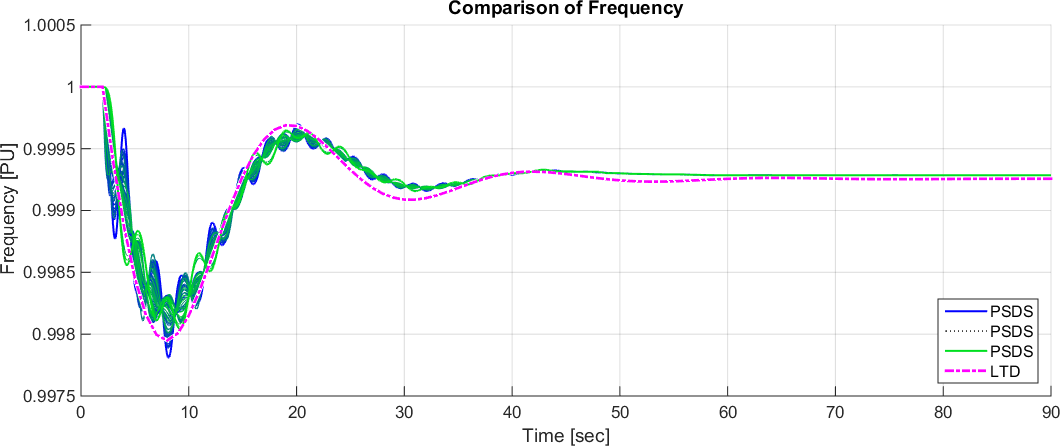
\includegraphics[width=\figW\linewidth,height=\figH\textheight]{fcomp.png}\vspace{-1em}
			\caption{All PSDS bus frequencies and LTD system frequency response.}
			\label{fcomp}		 
	\end{figure}\vspace{-2em}
	\begin{figure}[h!]
				\centering
				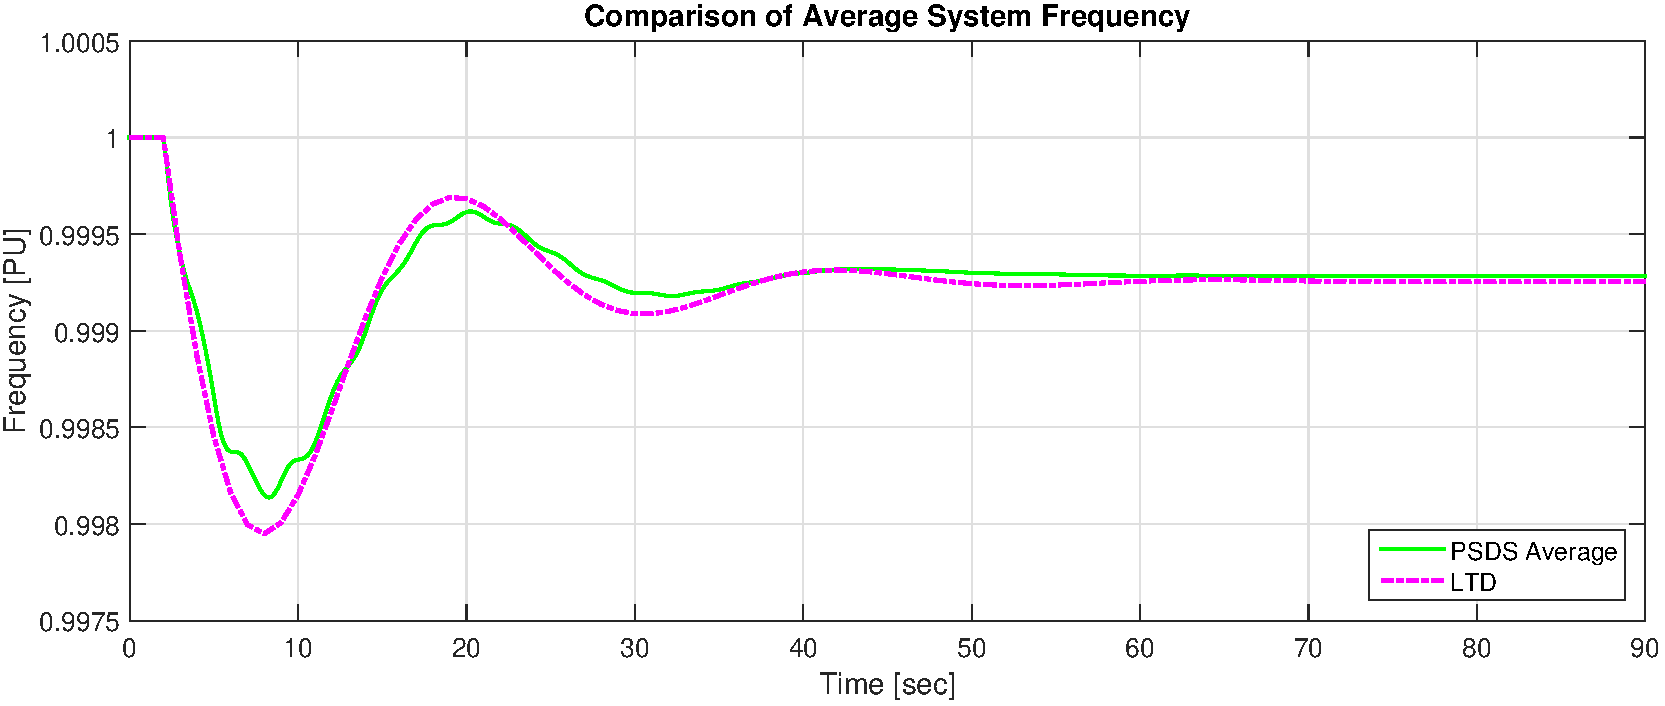
\includegraphics[width=\figW\linewidth,height=\figH\textheight]{aveFg}  \vspace{-2em}
				\caption{Averaged PSDS system response against LTD frequency. (Difference at $t(90) \approx$ 2.84E-5).} 
				\label{aveF}
	\end{figure}\vspace{-2em}
	\begin{figure}[h!]	
				\centering
				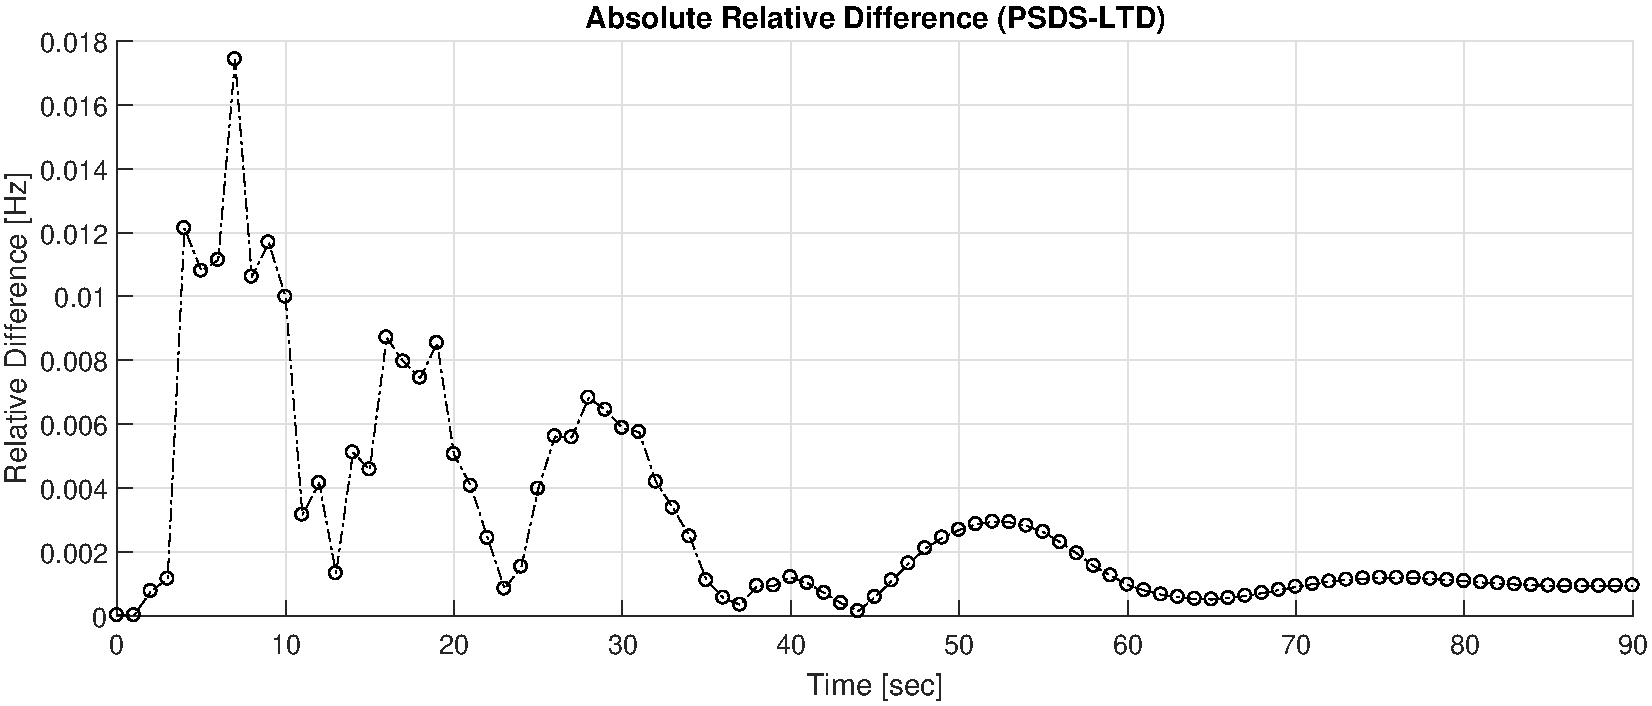
\includegraphics[width=\figW\linewidth,height=\figH\textheight]{relDif}  \vspace{-1.5em}
				\caption{Relative Hz difference of PSDS - LTD $\left( \text{i.e. }  \left|\dfrac{f_{PSDS}(t)- f_{LTD}(t)}{f_{PSDS}(t)}\right| \times 60 \text{Hz} \right)$.}
				\label{redDif}
	\end{figure}

\pagebreak
\begin{minipage}{.3\linewidth}
\paragraph{MiniWECC Model:}
\begin{description}
\item[Buses] 120
\item[Generators] 34
\item[Loads] 23
\item [Generation] 107,509 MW
\item[Load] 105,985 MW
\end{description}
\end{minipage}       
\hspace{3em}
\begin{minipage}{.5\linewidth}
\paragraph{Simulation Results (60 Second Run): } \

\begin{tabular}{r l l}
	& PSDS & LTD \\
Timestep & 4.167 ms & 1 sec \\
Produced Data File Size & 35,492 KB & 423 KB \\
Simulation Run Time & 41.42 sec & 11.75 sec \\
Speed up from PSDS & 1 & 3.52
\end{tabular}
\end{minipage}  
                 

\paragraph{Possible reasons for Steady State Variance} 
\subparagraph{1. Mishandled Machine Parameters:} PSDS and LTD Generator H and MWcap were verified as being the same for all machines in system.

\subparagraph{2. AMQP JSON message behavior:}
The coded AMQP procedure sends data as a json message and as shown below, a value with many decimals is rounded to be represented as a floating point (Line 6), and then truncated when added to a dictionary (Line 9). This rounded and truncated value is what is sent as the AMQP message (Line 11). Note that Python reports these values as the same (Lines 12-17). The \verb|numpy| (numerical python) package may have an alternate approach to this rounding / truncation behavior.

\begin{lstlisting}
>>> import json
>>> lval = 123.123456789012345678901234567890
>>> lval
123.12345678901235
>>> print('%.30f' % lval)
123.123456789012351464407402090728
>>> msg = {'mval': lval}
>>> msg
{'mval': 123.12345678901235}
>>> print(json.dumps(msg))
{"mval": 123.12345678901235}
>>> 123.123456789012345678901234567890-123.123456789012351464407402090728
0.0
>>> print('%.30e' % (123.123456789012345678901234567890 -  lval))
0.000000000000000000000000000000e+00
>>> 123.123456789012345678901234567890 ==  123.12345678901235
True
\end{lstlisting}

\subparagraph{3. Slack Tolerance:}
Decreasing the slack tolerance to 0.001 MW ( from 1 MW) had no effect on relative difference - though did increase simulation time by $\approx$7x due to the number of power flows required to solve each time step.

\subparagraph{4. Simulation Length:}
The simulation was run for 120 seconds and relative difference was found to vary slightly over time but stay between 3.3E-3\% and 2.1E-3\%.
\subparagraph{5. Integration method} Euler and RK-45 were found to have similar results and did not change relative difference.

\pagebreak
\paragraph{6. Differences in load distribution:} As shown in Figure \ref{pmnorm}, the steady state mechanical output does not change by the same amount in the two simulation environments. 
	\begin{figure}[h!]
			\centering
			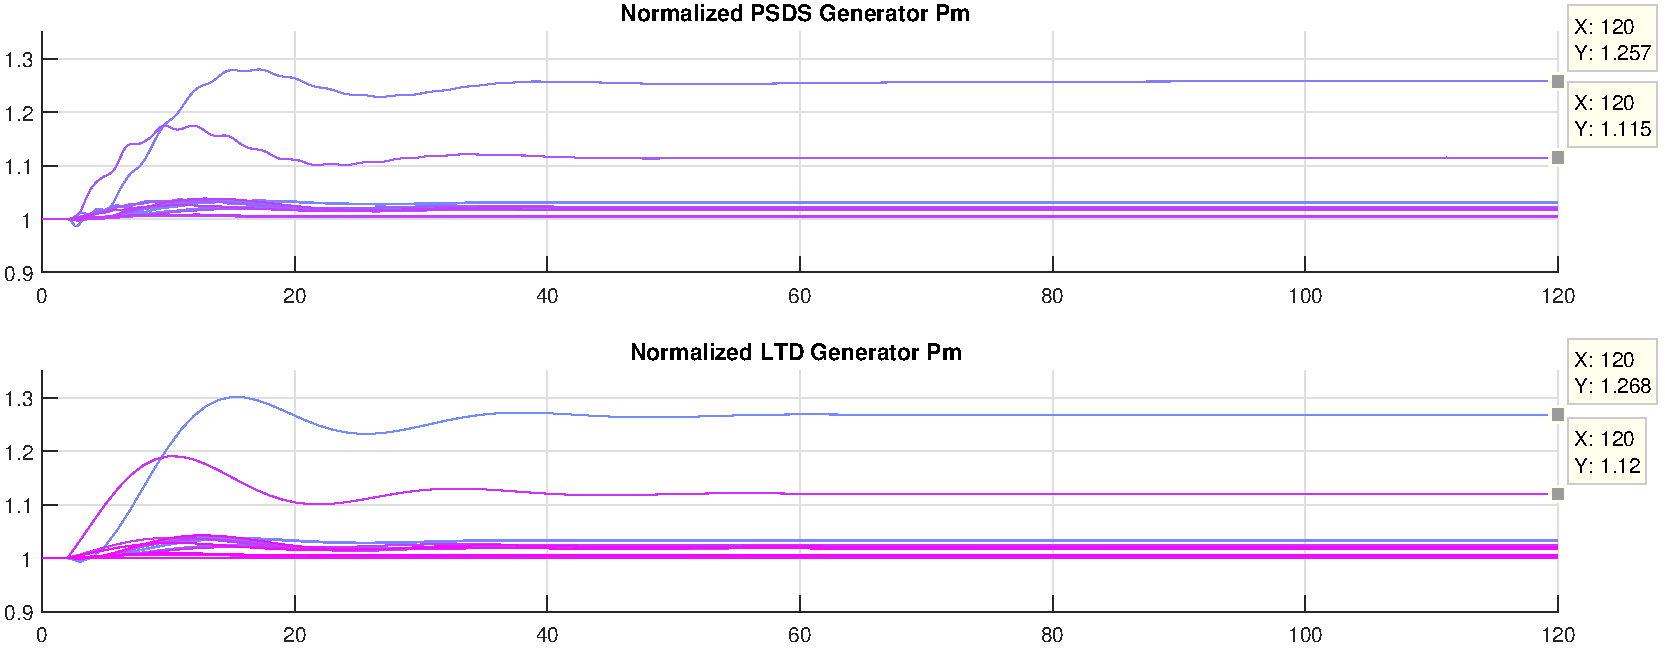
\includegraphics[width=\linewidth]{nomalizedPM}\vspace{-1em}
			\caption{Normalized $P_M$ from all machines in system. $\left( \text{i.e. }\dfrac{P_m(t)}{P_m(0)} \right)$}
			\label{pmnorm}		 
	\end{figure}\vspace{-.5em}

The table below quantified this difference for the two generators that had the largest \% change from $t(0)$.

\begin{table}[!ht]
	\centering
	\begin{tabular}{@{} lrrrr @{}} 	
		\toprule % @ signs to remove extra L R space
		\footnotesize % this will affect the table font (makse it 10pt)
		 Generator & PSDS  & LTD  & \% $\Delta$ Dif. & MW Dif.  \\
		\midrule		
		WA-GEN (slack top line) & 1.257  & 1.115  & 0.011   & 5.1\\
		SDG GEN (lower line) & 1.115  & 1.120  & 0.005 & 2.2 \\
		\bottomrule
	\end{tabular}

\end{table}

	\begin{figure}[h!]
			\centering
			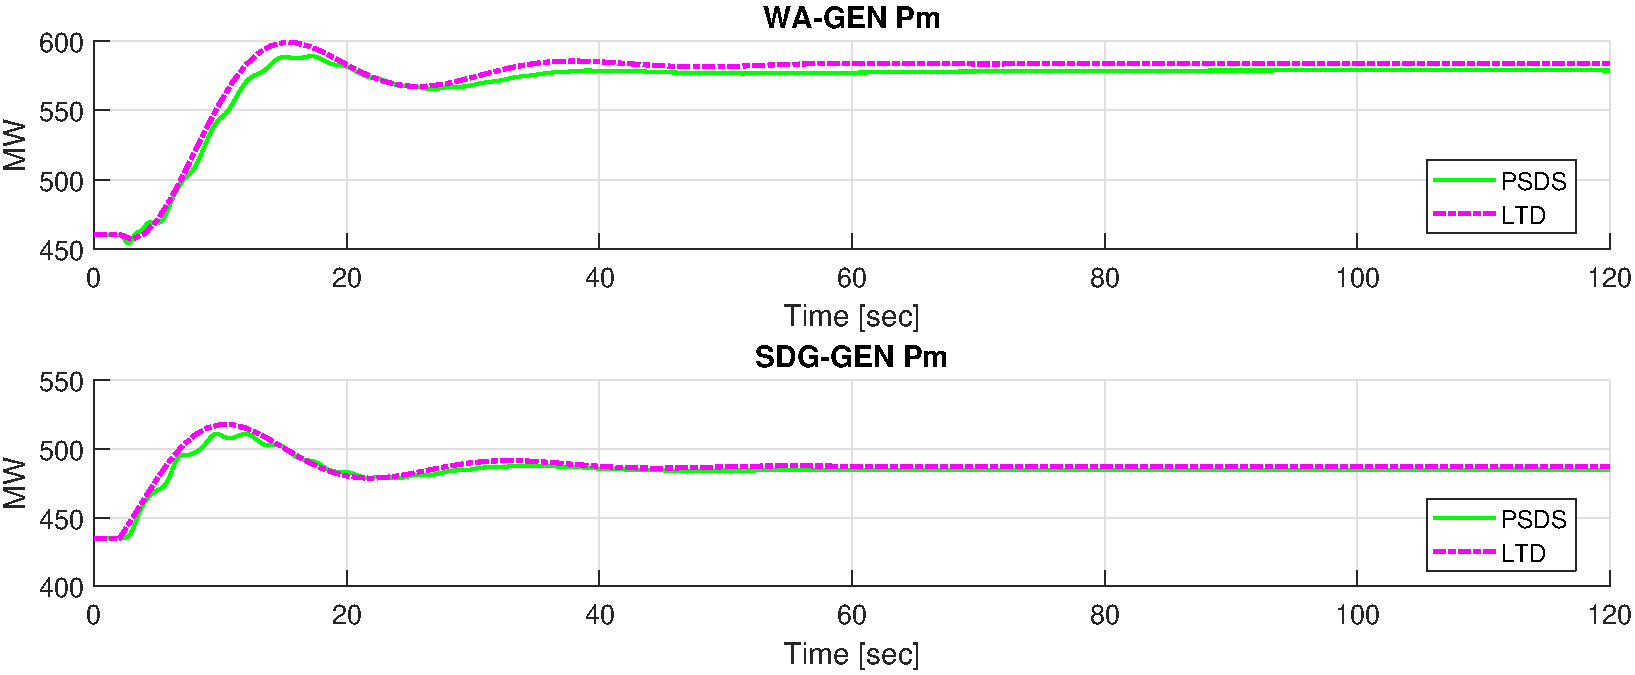
\includegraphics[width=\linewidth]{pmCompare}\vspace{-1em}
			\caption{$P_M$ from the machines that changed the most from $t(0)$.}
			\label{pmCompare}		 
	\end{figure}\vspace{-.5em}

\pagebreak
\paragraph{7. Time step resolution:} NOTE: Code changed after all previously listed test were ran.

Changing the time step affects accuracy, size of data collected, and simulation run time. The following data was collected from a 90 second simulation. LTD uses rk45 integration and 0.5 MW slack tolerance --- it is also run from the command line.The PSDS system has exciters and PSS included in dyd file.
Theoretical steady state frequency was calculated as 

$f = 1+\Delta f = 1 + \frac{\Delta P}{S_{base}\beta} = 1 + \frac{-1200 MW}{100 \times 15,555} = 0.999228543876567 = 59.953712632594019 Hz  $

\begin{table}[!ht]
	\centering
	\footnotesize % this will affect the table font (makse it 10pt)
	%\STautoround{2}
\renewcommand\STprintnum[1]{\numprint{#1}}
 \nprounddigits{2}

	\npthousandsep{,}
	\npdecimalsign{.}
	\begin{spreadtab}{{tabular}{lrrrrrrr}}
		\toprule % @ signs to remove extra L R space
		  & @Time step  & @\shortstack{Simulation\\ Time [sec] } &@ \shortstack{Data File \\Size [KB] }  &@ \shortstack{Real time \\Speed up}& @\shortstack{ PSDS\\Speed up} & @\shortstack{Reduction \\ of file size}  & @ \shortstack{Steady State  \\ $f$ error [Hz]}\\
		\midrule		
		@PSDS	& @4.167 ms 		&  56.12   	& 35070 	& \STcopy{v}{90/C2}		& 1 					& 1 					& @ 0.0034\\
		@LTD		&@	2 sec		& 9.41   	&	300 	& 	 					& \STcopy{v}{56.12/c3} 	& \STcopy{v}{!d!2/d3}	& @ 0.0017 \\ % miniWECC_loadStep01F.mir
		@LTD		&@	1 sec		& 17.39   	&	496 	&  						&  						& 						& @ 0.0017 \\ % miniWECC_loadSte@ p02F.mir
		@LTD		&@	0.5 sec		& 33.05   	&	888 	&  						&  						& 						& @ 0.0017\\ % miniWECC_loadStep03F.mir
		@LTD		&@	0.25 sec	& 63.67   	&	1672 	&   					&  						& 						& @ 0.0017\\ % miniWECC_loadStep04F.mir
		\bottomrule
	\end{spreadtab}
\end{table} 
\vspace{-1em}

	\begin{figure}[h!]
			\centering
			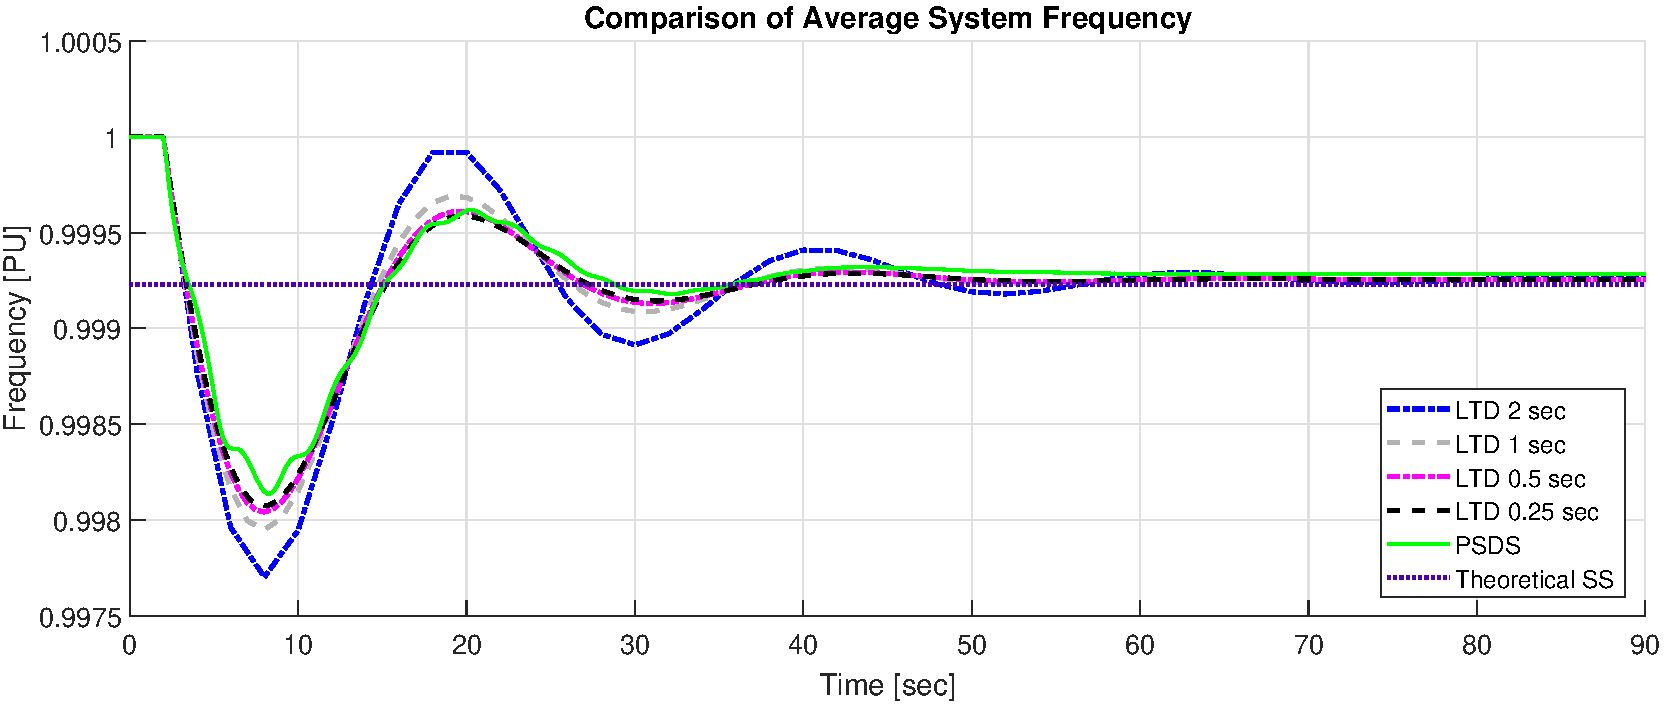
\includegraphics[width=\linewidth]{tsComp}\vspace{-1em}
			\caption{Comparison of system frequency among different time steps.}
			\label{tsComp}		 
	\end{figure}\vspace{-.5em}

	\begin{figure}[h!]
			\centering
			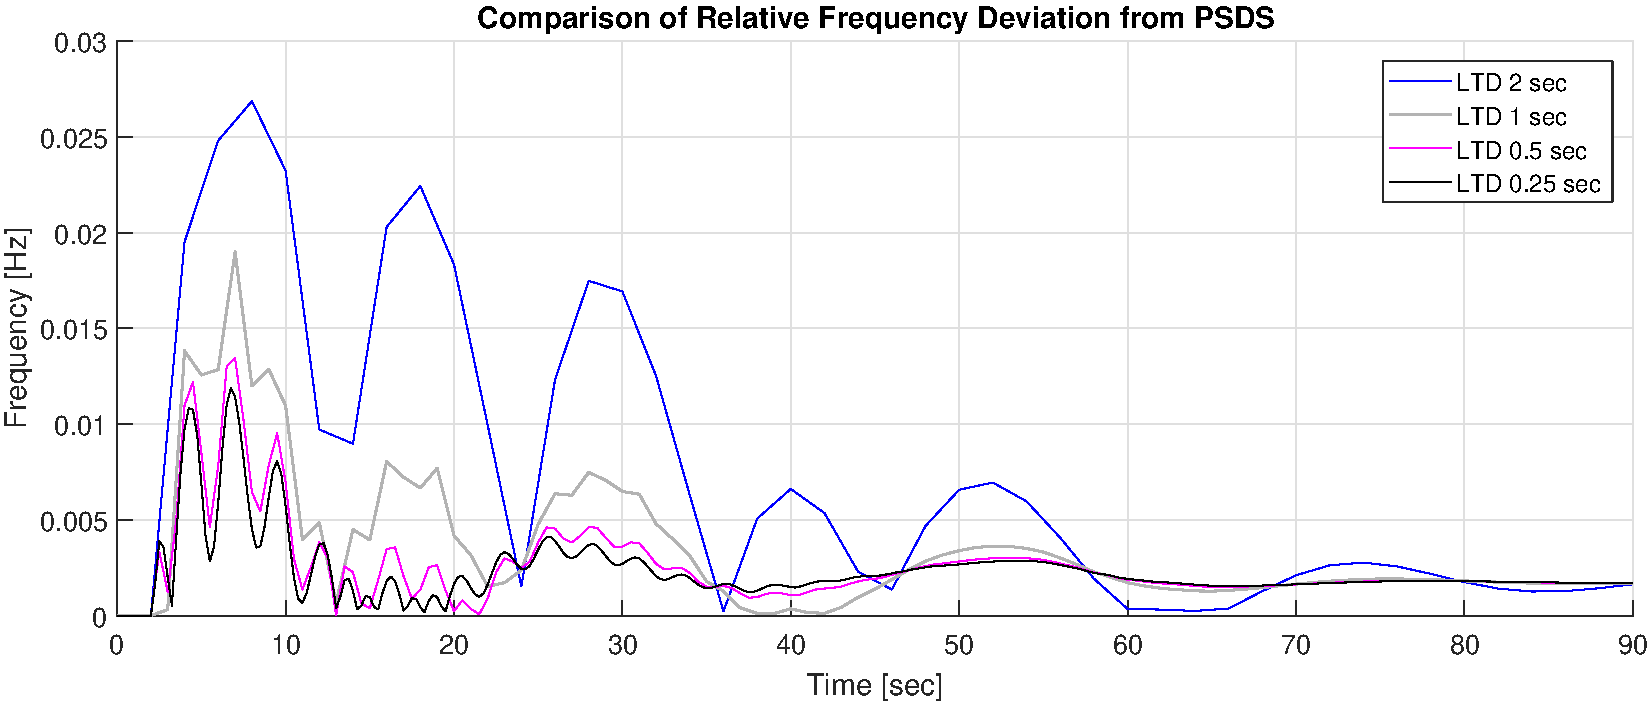
\includegraphics[width=\linewidth]{tsCompRelF}\vspace{-1em}
			\caption{Relative Hz difference of PSDS - LTD $\left( \text{i.e. }  \left|f_{PSDS}(t)- f_{LTD}(t)\right| \times 60 \text{Hz} \right)$.}
			\label{tsComprelF}		 
	\end{figure}\vspace{-.5em}

\end{document}
